% Created 2018-05-09 Wed 17:14
% Intended LaTeX compiler: pdflatex
\documentclass[12pt]{article} 
           \usepackage[labelfont=bf]{caption}
           \usepackage{times}


\usepackage{graphicx}
\usepackage{textcomp}
\usepackage{setspace}
\usepackage{amsmath}
\usepackage{mathtools}
\usepackage{cite}
\usepackage[labelfont=bf]{caption}
\usepackage{times}
\usepackage[T1]{fontenc}
\graphicspath{{../output/figures/}{../lib/}}
\topmargin 0.0cm
\oddsidemargin 0.2cm
\textwidth 16cm
\textheight 21cm
\footskip 1.0cm
\DeclarePairedDelimiterX{\infdivx}[2]{(}{)}{%
#1\;\delimsize\|\;#2%
}
\newcommand{\infdiv}{D_{KL}\infdivx}
\DeclarePairedDelimiter{\norm}{\lVert}{\rVert}
\newcommand\sumin{\sum_{i=1}^{n}}
\newcommand{\Xoi}[1]{#1(i)}
\newcommand{\frakPQ}[2]{\frac{\Xoi{#1}}{\Xoi{#2}}}
\newcommand{\DKLPQ}[3]{D_{\mathrm{KL}}(#1 #3 #2)}
\author{
Philipp Homan,$^{1}$
H. Lee Lau,$^{1}$
Ifat Levy,$^{2}$
Candace M. Raio,$^{3}$
Dominik R. Bach,$^{4, 5}$\\
David Carmel,$^{6\ast}$
Daniela Schiller,$^{1\ast}$\\
\\
\normalsize{$^{1}$Department of Psychiatry,}
\normalsize{Department of Neuroscience, and }
\normalsize{Friedman Brain Institute,}\\
\normalsize{Icahn School of Medicine at Mount Sinai}\\
\normalsize{1470 Madison Ave, NY, NY 10029, USA.}\\
\normalsize{$^{2}$Departments of Comparative Medicine,}
\normalsize{Neuroscience and Psychology}\\
\normalsize{Yale University,}
\normalsize{New Haven, CT, USA.}\\
\normalsize{$^{3}$Department of Psychology, }
\normalsize{New York University}\\
\normalsize{6 Washington Place, NY, NY 10003, USA.}\\
\normalsize{$^{4}$Clinical Psychiatry Research}\\
\normalsize{Department of Psychiatry, Psychotherapy, }
\normalsize{and Psychosomatics}\\
\normalsize{University of Zurich, Zurich, Switzerland}\\
\normalsize{$^{5}$Wellcome Centre for Human Neuroimaging,}\\
\normalsize{12 Queen Square, London WC1N 3BG, UK}\\
\normalsize{$^{6}$Psychology Department, }
\normalsize{University of Edinburgh}\\
\normalsize{7 George Square, Edinburgh EH8 9JZ, UK.}\\
\\
\normalsize{$^{\ast}$These authors contributed equally}\\
\normalsize{$^{\ast}$Correspondence: daniela.schiller@mssm.edu}
\normalsize{or dave.carmel@ed.ac.uk}\\
\\
}
\date{2018-05-09 17:14}
\title{\textbf{Affective flexibility without perceptual awareness}}
\begin{document}

\maketitle
\doublespacing
\clearpage

\section*{Abstract}
\label{sec:org38dfeea}
Can we change our reactions to threat without being aware of it?
Environmental cues that predict threat constantly change - new threats
may arise while old ones cease to pose a risk. When consciously
perceiving such cues, we are able to flexibly update and shift threat
responses from one cue to another. Threat-conditioned stimuli that are
perceived without awareness can still elicit physiological defensive
reactions, but it remains unknown whether the complex learning involved
in affective flexibility - creating new threat associations while
suppressing old ones - can be accomplished without awareness. Here,
participants underwent classical threat conditioning, in which one of
two images was paired with an electric shock; halfway through the
experiment, contingencies were reversed and the shock was paired with
the other image. The images were presented under continuous flash
suppression, a technique allowing suppression of stimuli from awareness
for several seconds. Importantly, although the trial-by-trial
effectiveness of suppression varied across participants, parametric and
computational analyses show that this was independent of the reversal
learning evident in physiological (skin conductance) responses:
dynamic updating - shifting reactions from a stimulus that no
longer predicts threat to one that now does - was accomplished
regardless of individual levels of perceptual awareness. In addition,
baseline anxiety levels scaled negatively with the strength of this
updating, consistent with previous reports of heightened anxiety
impeding learning. Our findings provide convincing evidence that the
successful updating of acquired threat responses does not require
perceptual awareness.

\textbf{Keywords}: fear conditioning; perceptual awareness; reversal learning;
unconscious processing; anxiety; continuous flash suppression

\clearpage

\section*{Significance statement}
\label{sec:orge3b4967}
In an ever-changing environment, survival depends on learning which
stimuli represent threat, and on updating such associations when
circumstances shift. This is a complex process: novel responses must be
generated while simultaneously suppressing learned ones. The role of
awareness in this affective flexibility remains unknown, and has major
implications for theories of both learning and consciousness. Humans can
acquire physiological responses to threat-associated stimuli even when
they are unaware of them; but we don't know whether the task of updating
such learning, previously shown only with awareness, can be accomplished
without it. Here, we show that it can, and furthermore, that human
physiological responses reflect changes in stimulus-threat pairings
independently of stimulus awareness, demonstrating the sophistication of
unconscious affective flexibility.

\clearpage

\section*{Introduction}
\label{sec:orgf00f222}
Flexible responses to environmental threats are essential for adaptive
behavior. This involves learning to respond to stimuli that signal
threat, but also the ability to update such responses if environmental
contingencies change - new threats may arise while old ones cease to
pose a risk. It is well established that learned defensive responses can
be updated when danger is consciously perceived
\cite{Morris2004,Schiller2008,Fleming2012} - physiological reactions
shift from a stimulus that no longer predicts danger to one that now
does. But can we update our reaction to stimuli that predict danger when
we are not even aware of them? Stimuli previously associated with an
aversive outcome can elicit physiological arousal when they are
suppressed from awareness
\cite{Critchley2002,Morris1998,Ohman1994,Whalen1998}, and new threat
associations can be formed through classical conditioning even without
any awareness of the conditioned stimuli
\cite{Katkin2001,Manns2002,Raio2012,Wiens2003}; however, it remains
unknown whether the complex process of updating threat learning requires
awareness of the stimuli, or can be accomplished without it. Here we
show that it can, and furthermore, that stimulus awareness does not seem
to play a substantial role in such affective flexibility.

To examine this, we employed the reversal paradigm, a laboratory model
that requires flexible updating of threat contingencies
\cite{Schiller2008}. In an initial acquisition phase, participants
encounter two conditioned stimuli (CSs) and learn that only one of them
predicts an electric shock. Halfway through the experiment, with no
warning, these contingencies flip, initiating the reversal phase:
Participants must flexibly learn that the formerly safe CS now predicts
the shock and that the old one no longer does. To assess learning,
participants' physiological arousal is recorded throughout the
experiment, typically (and here) by measuring their skin conductance
responses. Appropriate response reversal requires a sophisticated form
of updating, in that one must learn to respond to a cue that now
predicts threat while simultaneously inhibiting responses to the
previously threatening cue that is now safe.

To see whether reversal of conditioned threat requires awareness, we had
a large group of participants (\emph{N} = 86)
undergo reversal learning with the CSs suppressed from awareness by
continuous flash suppression (CFS), a technique commonly used to examine
unconscious perception
\cite{Raio2012,Tsuchiya2005,Stein2011,Carmel2010}: The CSs were visual
images presented monocularly, while the other eye was shown a
high-contrast, dynamic image (the CFS mask) at the corresponding retinal
location (See Figure \ref{fig:org8bbeaee} for a description of the design and
procedure).

CFS can suppress images from awareness for several seconds. However, it
is also known that its effectiveness may vary across trials and
individuals, and the suppressed stimulus may "break through" the
suppression \cite{Gayet2017}. Over the last decade, a growing body of
work has raised concerns that the standard approach - removing from
analysis data (participants and trials) in which break trough had
occurred - may bias the findings (\cite{Shanks2016,Stein2014a}; See
Supplementary Methods for further details of these issues.) Here, we
adopt a number of methodological approaches to ensure our results are
robust to these potential concerns.

Specifically, we remove no data and instead incorporate individual
levels of reported stimulus awareness, as well as response patterns that
might reflect residual awareness into a regression model accounting for
physiological responses. The model also adjusts for baseline anxiety
(which has been previously shown to correlate with unconscious learning;
\cite{Raio2012}). Additionally, we use a Bayesian approach to
establish that a model in which participants were updating their
learning provides a better account for the findings than a model in
which they were simply (and independently of the stimulus) predicting
the probability of a shock on the next trial. Finally, to verify that
reversal learning can be induced with awareness of our stimuli, we ran a
no-CFS group (\emph{N} = 12),
in which participants also viewed the CSs monocularly, but were aware of
them as no CFS masks were presented to their other eye.

We hypothesized that physiological responses to threat can be flexibly
reversed without perceptual awareness. We find that CS awareness is
indeed very weakly associated with reversal, and that there is strong
evidence for the reversal of threat learning even in its complete
absence.

\section*{Results and Discussion}
\label{sec:org85e499c}
\subsection*{Overall assessment of physiological reversal learning}
\label{sec:orgd4d269a}
To assess the physiological arousal evoked by CSs, we used a model-based
approach \cite{Bach2010} to estimate the amplitude of anticipatory
sudomotor nerve activity (SNA) from skin conductance data recorded
during stimulus presentation. A variational Bayes approximation was
employed to invert a forward model that describes how hidden SNA
translates into observable SCRs (see Materials and Methods). Previous
work has shown that this approach is more sensitive than conventional
SCR peak-to-peak analysis \cite{Bach2010,Bach2014,Staib2015}. Figure
\ref{fig:org8bbee4d}A shows the time course of evoked SNA to Spiders A and B,
separately for the CFS and no-CFS groups. In both groups, responses to
Spider A relative to Spider B were larger during the acquisition phase
and smaller during the reversal phase. To quantify the magnitude of
physiological reversal learning, we calculated a reversal learning index
for each participant (see Materials and Methods). The reversal learning
index was positive (indicating successful reversal) and significantly
greater than zero for both the CFS and no-CFS groups (Figure
\ref{fig:org8bbee4d}B).

Specifically, a linear mixed model (see Materials and Methods for
details) revealed a significant interaction of stage and spider in both
groups (CFS: \(\beta\) = 0.27, \emph{t} (2935) = 4.23, \emph{P} = < 0.001; no-CFS:
\(\beta\) = 1.23, \emph{t} (2935) = 7.29, \emph{P} = < 0.001); the interaction was stronger in the
no-CFS group than the CFS group (interaction of group, stage, and
spider; \(\beta\) = -0.96, \emph{t} (2935) = -5.35, \emph{P} = < 0.001). Note that a significant
interaction is formally equivalent to a significant reversal learning
index. These results indicate that
reversal learning was evident in both groups, and more pronounced in the
no-CFS group.

As previous work has found a negative association between anxiety and
threat acquisition with and without awareness \cite{Raio2012}, we also
calculated correlations between the CFS group's baseline anxiety
measures (STAIT, STAIS, FSQ) and the reversal learning index. Overall,
reversal learning decreased significantly with increasing levels of
state and trait anxiety, and to a lesser but non-significant extent for
spider phobia (Figure \ref{fig:org8bbee4d}C).

\subsection*{Reversal learning and perceptual awareness}
\label{sec:org24b6bb4}
The CFS manipulation reduced awareness of the CSs; as expected, however,
it was differentially effective in doing so across participants,
precluding an overall conclusion that all learning under CFS happened
non-consciously. The CFS group showed significantly lower accuracy in
response to the "which seen?" question (M = 0.46, SD = 0.29) compared to the no-CFS
group (M = 0.86, SD = 0.16; \emph{t} (22.77) = -7.24, \emph{P} < 0.001), and accuracy in the CFS group was not
significantly different from the 50\% random-response level
(\emph{t} (85) = -1.21, \emph{P} = 0.229). The CFS group also showed lower confidence
(M = 1.73, SD = 0.65) than the no-CFS group (
M = 2.83, SD = 0.08; 
\emph{t} (95.38) = -15.05, \emph{P} < 0.001).

However, group differences in accuracy and confidence, and even
random-level response accuracy, are not sufficient to establish an
absence of perceptual awareness in the CFS group. Notably, average
confidence of correct responses in this group was low but significantly
greater than the minimum value of 1 (
\emph{t} (77) = 10.79, \emph{P} < 0.001), suggesting that at least
some participants were aware of some of the CSs; learning might thus
have arisen from a subset of trials and/or participants where such
awareness occurred. To address this, we quantified CS awareness by
calculating an awareness index for each participant, ranging in possible
values from 0 for no awareness to 1 for full awareness (see Materials
and Methods). Although the awareness index of the CFS group
(M = 0.28, SD = 0.34)
was significantly lower than the no-CFS group's
(M = 0.92, SD = 0.18; \emph{t} (23.93) = -10.19, \emph{P} < 0.001), it was still significantly higher than zero
(\emph{t} (85) = 7.59, \emph{P} < 0.001).

Therefore, in order to test our main hypothesis that the reversal of
acquired threat responses can be achieved without perceptual awareness,
we characterized the quantitative relation between the level of
awareness and the magnitude of reversal learning. To control for
possible artifacts of regression to the mean (see Supplementary
Methods), we first calculated the correlation between two independent
estimates of the awareness index \cite{Shanks2016}, one calculated
from even-numbered trials, the other from odd-numbered trials. These
measures were strongly correlated (
\emph{r} (84) = 0.96, \emph{P} < 0.001; Figure
\ref{fig:orgd1537f6}A); participants' awareness level in one set of trials
was thus overwhelmingly predictive of their awareness in the other set,
demonstrating the reliability of the awareness measure and indicating
that an individual's overall awareness index was unlikely to have an
extreme value that was due to measurement-level noise.

Next, we examined the association between the reversal learning index
and the awareness index, using values of both indices obtained
separately from even (Figure \ref{fig:orgd1537f6}B) and odd (Figure
\ref{fig:orgd1537f6}C) trials. As the color-coding of Figure
\ref{fig:orgd1537f6} shows, the relation between individual participants'
reversal learning and their awareness was highly consistent across these
separate measurements. In light of this, we pooled the data from all
trials and regressed the reversal learning index on the perceptual
awareness index (Figure \ref{fig:orgd1537f6}D). The parameter of interest
was the intercept, which corresponds to the magnitude of reversal
learning at zero perceptual awareness. The intercept was positive and
significantly different from zero, and furthermore, the awareness index
regressor did not contribute significantly to prediction of reversal
learning; importantly, this finding was even stronger in models that
accounted for STAIT scores and a binary factor indicating whether
participants were tracking the stimuli with their responses (see
Materials and Methods; Figure \ref{fig:orgd1537f6}E and Table
\ref{tab:org3572c3f}).

\subsection*{Comparing learning and expectation-based accounts}
\label{sec:orgae0bf98}
Well-controlled lab-based conditioning procedures require strict
constraints that preclude complete randomization of the number and order
of different CSs; this comes with a cost: participants are able to
develop expectations with above-chance validity, based on the sequence
of trials so far, about the likelihood of a shock on any upcoming
trial. Even without any awareness of the CSs, a participant should have
been able to distinguish two types of trials: reinforced (with shock)
and non-reinforced (no-shock). In a study with two CSs and a 100\%
reinforcement rate like ours, such expectations would correspond to an
anticipated pattern of alternating trial-types (shock/no-shock or vice
versa), with an increase in shock anticipation after every no-shock
trial. The question, therefore, was whether the physiological responses
we had measured might simply reflect participants' pattern-based
anticipation of shock, rather than learning of the contingencies
associated with the CSs.

To answer this question, we used a Bayesian approach to compare the
probability of our findings being accounted for by a classic
Rescorla-Wagner learning model \cite{Rescorla1972} and a
trial-sequence model. We hypothesized that successful threat reversal
without perceptual awareness should be better explained by the
Rescorla-Wagner learning model, whereas simple pattern-based expectation
would be better explained by the trial-sequence learning model. We used
maximum likelihood estimation to assess the log likelihood and calculate
the Bayesian Information Criterion (BIC) of each model (See Materials
and Methods for details of each model and calculation of the BIC). A
smaller BIC indicates a better model, and BIC values can thus be
compared by calculating the difference between them and interpreting the
resulting \(\Delta\) BIC as providing evidence against the higher BIC. The
Rescorla-Wagner model (BIC: 562.1) outperformed the pattern-based
expectation model (BIC: 584.9), with the difference (\(\Delta\) BIC: 22.9)
greater than 10, suggesting that the evidence against the trial
switch model is very strong \cite{Raftery1995}. Repeating this
comparison for just the participants with zero mean awareness confirmed
the lower BIC for the Rescorla-Wagner model (BIC: 114.3) compared to the
pattern-based expectation model (BIC: 125.7), with the difference again
greater than 10 (\(\Delta\) BIC: 11.3; see also
Figure S\ref{fig:org918e8f8}). This model comparison provides convincing
evidence that a classical Rescorla-Wagner learning model explains our
findings better than an alternative expectation-based model.

These results indicate that participants were able to update their
defensive physiological responses independently of their awareness of
threat-related cues. Previous studies have shown that new threat
associations can be formed without perceptual awareness of the
conditioned stimuli
\cite{Manns2002,Wiens2003,Morris1998,Raio2012}. However, until now it
was unknown whether the far more complex process of threat reversal -
shifting reactions from a stimulus that no longer predicts danger to one
that now does - can be accomplished without awareness.  Our finding of
reversal learning occurring independently of the level of perceptual
awareness suggests that separate processes underlie affective
flexibility and conscious processing \cite{Lau2011}. Conversely, the
negative correlation between reversal learning and anxiety suggests that
the various impairments caused by anxiety are not limited to systems
underlying conscious processes.

Previous studies have pointed out the limitations of using accuracy and
confidence measures to assess perceptual awareness, and suggested
remedies including the calculation of metacognitive sensitivity measures
\cite{Fleming2014}, Bayesian statistics \cite{Dienes2015}, or
parametric variation of the experimental manipulation
\cite{Schmidt2015}. The present study addresses an issue not covered
in previous discussions, by showing that a trial-wise analysis may
reveal hints for incomplete suppression that analyses relying on average
measures might easily miss. Future studies that rely on forced-choice
questions for awareness assessment should thus examine response patterns
across trials in addition to collecting aggregate measures. 

The ability to reverse conditioned responses depends on the integrity of
circuitry spanning several neural regions, particularly the ventromedial
prefrontal cortex (vmPFC) and its connections with the
amygdala\cite{Morris2004} where threat associations are formed
\cite{Roy2012}. Consistent with this, it is known that patients with
anxiety disorders often show rigid and inflexible threat responses in
conjunction with prefrontal cortex dysfunction
\cite{Ressler2007,Rauch2006}. Indeed, the real-life settings that
people with anxiety disorders find challenging often require the
updating and shifting of threat responses. Deficits in affective
flexibility may thus explain the threat learning and extinction deficits
seen in such disorders \cite{Duits2015}. Compared to healthy controls,
patients are less able to distinguish between safe and unsafe stimuli in
threat learning (when it is adaptive to do so), and distinguish between
them to a greater extent during extinction (when it is
non-adaptive). Threat learning without perceptual awareness is also
negatively correlated with baseline state anxiety in healthy
participants \cite{Raio2012}. Our new finding that baseline anxiety is
negatively correlated with affective flexibility suggests a potential
use for reversal learning as a model paradigm for investigating how
anxiety modulates various processes in a variety of disorders,
including, for example, posttraumatic stress disorder, in which there is
an impairment of threat inhibition \cite{Jovanovic2011}.

\section*{Materials and Methods}
\label{sec:orgcd39cff}
\subsection*{Participants}
\label{sec:org2d2f2c5}
Ninety-eight healthy participants (mean age = 29.97; range 18-65) were
assigned to one of the two groups: reversal learning with CFS (CFS
group; \emph{N} = 86, 48 female) or without CFS (no-CFS group; \emph{N} = 12, 5
female). Assignment was random until each group reached a size of 12;
subsequent participants were assigned to the CFS group. Measures of
trait and state anxiety (Spielberger Trait-State Anxiety Inventory
\cite{Spielberger1983}; STAIT and STAIS, respectively) and spider
phobia (Fear of Spider Questionnaire; FSQ \cite{Szymanski1995}) were
taken prior to participation and did not differ between the groups
(Table S\ref{tab:org270f0e5}). The experiment was approved by the Institutional
Review Board of the Icahn School of Medicine at Mount Sinai. All
participants provided written informed consent and were financially
compensated for their participation.

\subsection*{Experimental procedure}
\label{sec:orga739576}
Participants viewed the stimuli monocularly, through a mirror
stereoscope (StereoAids, Australia) placed at a distance of 45 cm from a
17-inch Dell monitor. The CSs (schematic low-contrast images of
spiders), presented to the left eye only, were suppressed from awareness
in the CFS group: while the left eye saw them, the right eye was
presented with "Mondrians" - arrays of high contrast, multi-colored,
randomly generated rectangles alternating at 10 Hz. Both the CSs and the
CFS masks were flanked by identical textured black and white bars, to
facilitate stable ocular vergence. The no-CFS group viewed identical CSs
(also presented monocularly), but with no Mondrians presented to the
other eye.

The experiment consisted of 16 acquisition trials followed by 16
reversal trials. One of two spider images was presented on each
trial. During acquisition, spider A always terminated with a shock and
spider B never did. Reversal occurred halfway through the experiment:
spider B now terminated with a shock and spider A did not. The spider
stimuli were presented for 6 s each in pseudorandomized order. One of
four possible trial orders was used for each participant. Orders were
generated by imposing specific constraints on the trial order, such that
the first trial was always reinforced and no more than two of the same
trial type ever occurred consecutively.

Trial order and spider identity were counterbalanced across
participants. To assess the effectiveness of the awareness
manipulation \cite{Merikle2001}, 1 s after the offset of every CS
participants were shown the question "Which seen?" (1 = flower, 2 =
spider; notably, flowers were never shown, meaning the question
addressed detection rather than discrimination as it could be answered
correctly even with a brief glimpse). This was followed by the question
"How confident?" (1 = guess to 3 = sure; participants were instructed to
indicate how confident they were of the flower/spider answer they had
just given). Both questions were presented binocularly (1.5 - 2 s each,
during which responses had to be given by pressing number keys on a
standard keyboard). The second question was followed by an 8 to 10 s
inter-trial interval.

\subsection*{Psychophysiological stimulation and measurement}
\label{sec:org3083f09}
Mild electric shocks were delivered using a Grass Medical Instruments
SD9 stimulator and stimulating bar electrode attached to the
participant's right wrist. Shocks (200ms; 50pulse/s) were delivered at a
level determined individually by each participant as "uncomfortable but
not painful" (maximum of 60V), during a work-up procedure prior to the
experiment.  

Skin conductance responses (SCR) were measured with Ag-AgCl electrodes,
filled with standard isotonic NaCl electrolyte gel, and attached to the
middle phalanges of the second and third fingers of the left hand. SCR
signals were sampled continuously at a rate of 200 Hz, amplified and
recorded with a MP150 BIOPAC Systems skin conductance module connected
to a PC.

\subsection*{Analysis of physiological responses}
\label{sec:org63ea6a0}
\subsubsection*{Model-based analysis}
\label{sec:org6f85e1c}
We estimated SNA from SCR data with a model-based variational Bayes
approximation \cite{Bach2010}, inverting a forward model that
describes how (hidden) SNA translates into (observable) SCR. A unit
increase in SNA corresponds to an increase in SCR of 1 micro
Siemens. The model assumes that the observed SCR can be decomposed into
different components including anticipation, evocation, and spontaneous
fluctuations, each of which are generated by bursts of SNA driven by
changes in sympathetic arousal. The generative (forward) model thus
describes how sympathetic arousal, the physiological measure that is
taken as an index of the psychological process of threat, translates
into sudomotor nerve bursts which then generate the observable SCR
\cite{Bach2010}. Using Bayesian inference, the forward model can then
be reversed in order to estimate the most likely underlying SNA given
the observed SCR:

\begin{equation}
p(\theta|y) = \frac{p(\theta)p(y|\theta)}{p(y)},
\end{equation}
where the most likely parameter vector \(\theta\) (corresponding to the SNA)
given the observed outcome \(y\) (corresponding to the SCR) is given by
the prior estimate of \(\theta\) weighted by the likelihood of \(y\) given
\(\theta\). Solving this equation involves integration over the model
evidence p(y) which is analytically hard to compute (and possibly
intractable). This can be resolved by replacing this integration problem
by an optimization problem, which can be approximated with Variational
Bayes procedures \cite{Friston2006a}, where the log of the model
evidence can be framed as the sum of the Kullback-Leibler divergence and
the Free Energy. By maximizing the Free Energy the Kullback-Leibler
divergence is minimized, and a lower bound to the log model evidence can
be derived iteratively.

The SNA estimates were computed using previously developed software
package PsPM \cite{Bach2010} implemented in MATLAB R2016b (The
Mathworks Inc, Natick, MA, USA). The statistical analyses were conducted
with the R software \cite{R-Core-Team2016}
(R version 3.4.2 (2017-09-28)) and the libraries lme4 \cite{Bates2005} and lsmeans
\cite{Lenth2016}. Welch's t-tests were used instead of two sample
t-tests when groups had unequal variances.

\subsubsection*{Reversal Learning Index}
\label{sec:orge7d4d66}
An estimate of SNA was obtained for each trial. We expected Spider A to
evoke greater SNA than Spider B during the acquisition phase, and Spider
B to evoke greater SNA than Spider A during the reversal phase. The
strength of reversal learning can thus be quantified by calculating,
separately for the acquisition and reversal phases, the difference
between the average SNA evoked by each spider. To quantify the degree of
reversal (which is formally equivalent to the interaction of phase and
stimulus), the reversal learning index was calculated by subtracting the
difference between mean SNAs evoked by each spider during reversal from
the difference during acquisition (the larger the index, the greater the
magnitude of reversal learning):

\begin{equation}
\begin{aligned}
  \text{Reversal learning index} &= \Delta \text{Acquisition} - \Delta \text{Reversal} \\
 \Delta \text{Acquisition} &= [\text{mean(Spider A)} - \text{mean(Spider B)}]_{\mathrm{Acquisition}} \\
    \Delta \text{Reversal} &= [\text{mean(Spider A)} - \text{mean(Spider B)}]_{\mathrm{Reversal}} 
\end{aligned}
\end{equation}
To formally test for group differences in the strength of reversal
learning, we computed a linear mixed model using the lme4 library in
R. We used the skin conductance response (converted to a model-based
measure of sudomotor nerve activity, SNA) as the dependent variable and
entered group (CFS, no-CFS), stage (acquisition, reversal), and spider
(spider A, spider B) as well as a continuous variable for trial (to
account for habituation) as predictors. The random structure of the
model included an intercept and slopes for stage and spider.

\subsection*{Assessments of perceptual awareness}
\label{sec:org0fbfc2f}
\subsubsection*{Perceptual awareness index}
\label{sec:org52ca384}
To characterize participants' reported awareness of CSs, each trial was
assigned a perceptual awareness score, defined by a combination of
detection and confidence responses: Correct answers with a confidence
rating of 1 (guess) and incorrect answers irrespective of confidence
were assigned an awareness score of 0; correct answers with a confidence
rating of 2 (medium) were assigned a score of 0.5, and correct answers
with a confidence rating of 3 (high) were assigned an awareness score
of 1. A perceptual awareness index was calculated for each participant
by averaging awareness scores across all trials.

\subsubsection*{Stimulus-response association patterns ("tracking")}
\label{sec:org36d4f2d}
We also assessed response patterns across trials, to see whether
participants were able to track stimuli with their responses, accurately
discriminating the images despite not being able to label them. We
plotted individual trial-by-trial responses to the question "Which
seen?", overlaid on the trial-by-trial presentation of spiders (spider
A, spider B; Figure S\ref{fig:orge0dadc6}A). We then calculated the number of
consecutive "hits", defined as the number of consecutive trials where
these two time-courses were either identical or consistently in
opposition, suggesting that there was a possible association between the
stimulus and the response during those trials. The probability of such
consecutive hits occurring by chance alone can be derived as follows:

Let \(p = 0.5\) be the probability of a hit, \(k\) the number of consecutive
hits, \(n\) the number of trials left, \(i\) the number of consecutive hits
already observed; the chance of observing \(k\) consecutive hits for the
remaining \(n\) trials can then be formulated as a recursive problem:
\begin{align}
f_{p, k}(i, n) = pf_{p, k}(i + 1, n - 1) + (1 - p) f_{p, k}(0, n-1),
\end{align}
which can be solved analytically with dynamic programming or recursion.
Trivially, \(f_{p, k}(k, n) = 1\) for \(n \geq 0\) since \(k\) consecutive
hits have already been observed, and \(f_{p, k}(i, n) = 0\) for \(k - i >
n\) since there are not enough trials left to observe \(k\) consecutive
hits.  

For example, assuming we want to know how likely it is to observe \(k =
8\) consecutive hits within \(n = 32\) trials given \(p = 0.5\), i.e.,
\(f_{0.5, 8}(0, 32)\), we find that this yields a probability of 0.050.

Alternatively, the probability can be derived by simulation for all
possible numbers of consecutive hits within 32 trials (i.e., from 1 to
31). For each possible number, we thus also simulated 10\(^{\text{5}}\) draws of a
binomial distribution and calculated the average probability of that
number of hits being consecutive. As can be seen in Figure
S\ref{fig:orge0dadc6}B, the result for 8 consecutive hits
(0.04991) was very close to the analytical
solution. Fifteen participants showed evidence of tracking the spiders
or the shocks with their responses (8 or more consecutive hits);
notably, 3 of these participants appeared to have a perceptual awareness
index of zero. We thus adjusted our subsequent analysis with an
additional binary covariate, indicating whether participants did or did
not show 8 or more consecutive hits.

\subsection*{Comparing learning and expectation-based models}
\label{sec:org536b900}
The Rescorla-Wagner model \cite{Rescorla1972} describes how the
prediction for each trial is updated according to a prediction error and
learning rate:

\begin{equation}
\begin{aligned}
V_{n+1}(x_{n}) &= V_{n}(x_{n}) + \alpha \delta_{n} \\
\delta_{n} &= r_{n} - V_{n}(x_{n}), \\
\end{aligned}
\end{equation}
where \(x_{n}\) is the conditioned stimulus on trial \(n\) (Spider A or
Spider B), and \(\delta_{\text{n}}\) is the punishment prediction error that
measures the difference between the expected and the actual shock
(\(r_{n}\)) on trial \(n\). The learning rate \(\alpha\) for the value update is
a constant free parameter. The value for the CS not observed on trial
\(n\) remains unchanged. To derive the best fits for the Rescorla-Wagner
model, we assumed that \(V_{0} = 0.5\), reflecting the assumption that
getting a shock or not was equally likely for the first trial.

For the alternative trial-sequence learning model, we assumed that a
participant expecting a strict sequence of alternating trial types
(shock/no shock or vice versa) would update this expectation according
to the actually encountered trial types and a constant learning rate:

\begin{equation}
\begin{aligned}
V'_{n+1} &= V'_{n} + \alpha' \delta'_{n} \\
\delta'_{n} &= r'_{n} - V'_{n} \\
\tau_{n} &= \lvert (r'_{n-1} - 1) \rvert, \\
\end{aligned}
\end{equation}
where \(V'_{n+1}\) is the expected trial type switch at trial \(n+1\) (if
\(V'_{n+1}\) is larger than 0.5, a trial switch is expected), \(\alpha'\) is
the learning rate, and \(\delta'_{n}\) is the prediction error. The
prediction error corresponds to the difference between the actual trial
type switch for trial \(n\) (\(r'_{n}\); coded as one for a trial type
switch and zero for an equal trial type) and the expectation for trial
n. A changing trial type for trial n was tracked by \(\tau_{n}\), which
was one if the preceding trial was zero and zero if the preceding trial
type was one. To map these expectations onto expected values, we assumed
that

\begin{equation}
\begin{aligned}
V_{n+1} &= 
\begin{cases}
V'_{n+1} \cdot \tau_{n} + (1 - V'_{n+1}) (1 - \tau_{n}), & \text{if } V' > 0.5 \\
V'_{n+1},                              & \text{otherwise},  
\end{cases}
\end{aligned}
\end{equation}
where the expected value for trial \(n+1\) was calculated according to
whether a trial type switch was expected (\(V' > 0.5\)) or not.  

We performed a formal model comparison between the conventional
Rescorla-Wagner model and the trial switch model for our data set
(Figure S\ref{fig:org918e8f8}), using maximum likelihood estimation and
non-linear optimization (implemented with the fmincon function in MATLAB
R2016b (The Mathworks Inc, Natick, MA, USA). Using the log likelihood,
we calculated the Bayesian Information Criterion (BIC) to compare the
two models as follows:

\begin{equation}
\begin{aligned}
\text{BIC} = \text{log}(n)\,k - 2 \cdot \text{log}(\hat{L}),
\end{aligned}
\end{equation}
where \(n\) is the number of data points, \(k\) is the number of regressors,
and \(\hat{L}\) is the maximized value of the likelihood function.

\section*{Acknowledgments}
\label{sec:org5121e1f}
All authors declare no conflicts of interest with regard to the current
study. We thank Patrik Vuilleumier who created and shared the spider
stimuli. This work was supported in part through the computational
resources and staff expertise provided by Scientific Computing at the
Icahn School of Medicine at Mount Sinai.  Funding was provided by NIMH
grant MH105515 and a Klingenstein-Simons Fellowship Award in the
Neurosciences to D.S.; ERC Advanced Grant XSPECT-DLV-692739 to D.C.
(Co-I); and Swiss National Science Foundation grant SNF 161077 to
P.H. The funding source had no role in the design and conduct of the
study; collection, management, analysis, and interpretation of the data;
preparation, review, or approval of the manuscript; and decision to
submit the manuscript for publication.

\clearpage

\bibliographystyle{pnas}
\bibliography{master}

\clearpage
\singlespace

\section*{Tables and Figures}
\label{sec:org83a81bf}
\singlespacing
\begin{table}[htbp]
\centering
\begin{tabular}{rlrrrr}
\textbf{Model} & \textbf{Predictor} & \textbf{Beta} & \textbf{SE} & \textbf{\emph{t}} & \textbf{\emph{P}}\\
\hline
1 & Intercept & 0.3 & 0.2 & 2.1 & 0.035\\
1 & Awareness index & -0.1 & 0.4 & -0.4 & 0.692\\
2 & Intercept & 1.4 & 0.5 & 3 & 0.004\\
2 & STAIT & 0 & 0 & -2.3 & 0.024\\
2 & Awareness index & -0.2 & 0.4 & -0.5 & 0.596\\
3 & Intercept & 1.5 & 0.5 & 3.1 & 0.003\\
3 & STAIT & 0 & 0 & -2.4 & 0.021\\
3 & Tracking score & -0.3 & 0.3 & -1 & 0.318\\
3 & Awareness index & -0.2 & 0.4 & -0.5 & 0.597\\
\end{tabular}
\caption{\label{tab:org3572c3f}
\textbf{Regression coefficients for all awareness index models.} Reversal learning was the dependent variable in all models. Model 1 included an intercept and the perceptual awareness index; model 2 additionally included STAIT scores; model 3 additionally included STAIT and tracking scores.}

\end{table}

\clearpage
\begin{figure}[htbp]
\centering
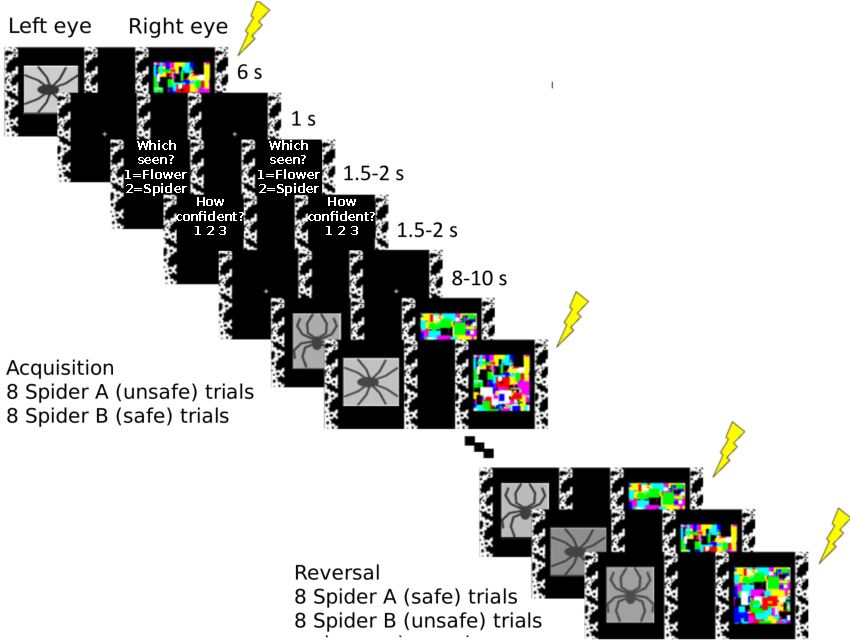
\includegraphics[width=0.9\textwidth]{cfs_revtask.pdf}
\caption{\label{fig:org8bbeaee}
\textbf{Experimental design and procedure.} In each trial of the acquisition phase, participants were presented with one of two stimuli (schematic pictures of spiders, presented monocularly for 6 sec and suppressed from awareness by a CFS mask shown to the other eye). One image (spider A) always terminated with a mild electric shock to the wrist, whereas the other (spider B) never did. Halfway through the experiment, with no warning, the contingencies flipped and the reversal phase began: the formerly safe stimulus (spider B) now predicted the shock, and the old threat-associated one (spider A) was now safe. Each spider was shown 8 times in each phase. Trial order was pseudorandomized (see Materials and Methods) and spider identity (A and B) was counterbalanced across participants. To assess the success of the awareness manipulation, participants answered the questions "Which seen?" (1=flower, 2=spider) and "How confident?" (1=guess to 3=sure), presented binocularly (1.5 - 2 s each), beginning 1 s after the offset of every CS, and followed by an 8-10 s inter-trial interval. Participants who underwent the same procedure without CFS were shown identical CSs, but the CFS mask was absent.}
\end{figure}

\clearpage
\begin{figure}[htbp]
\centering
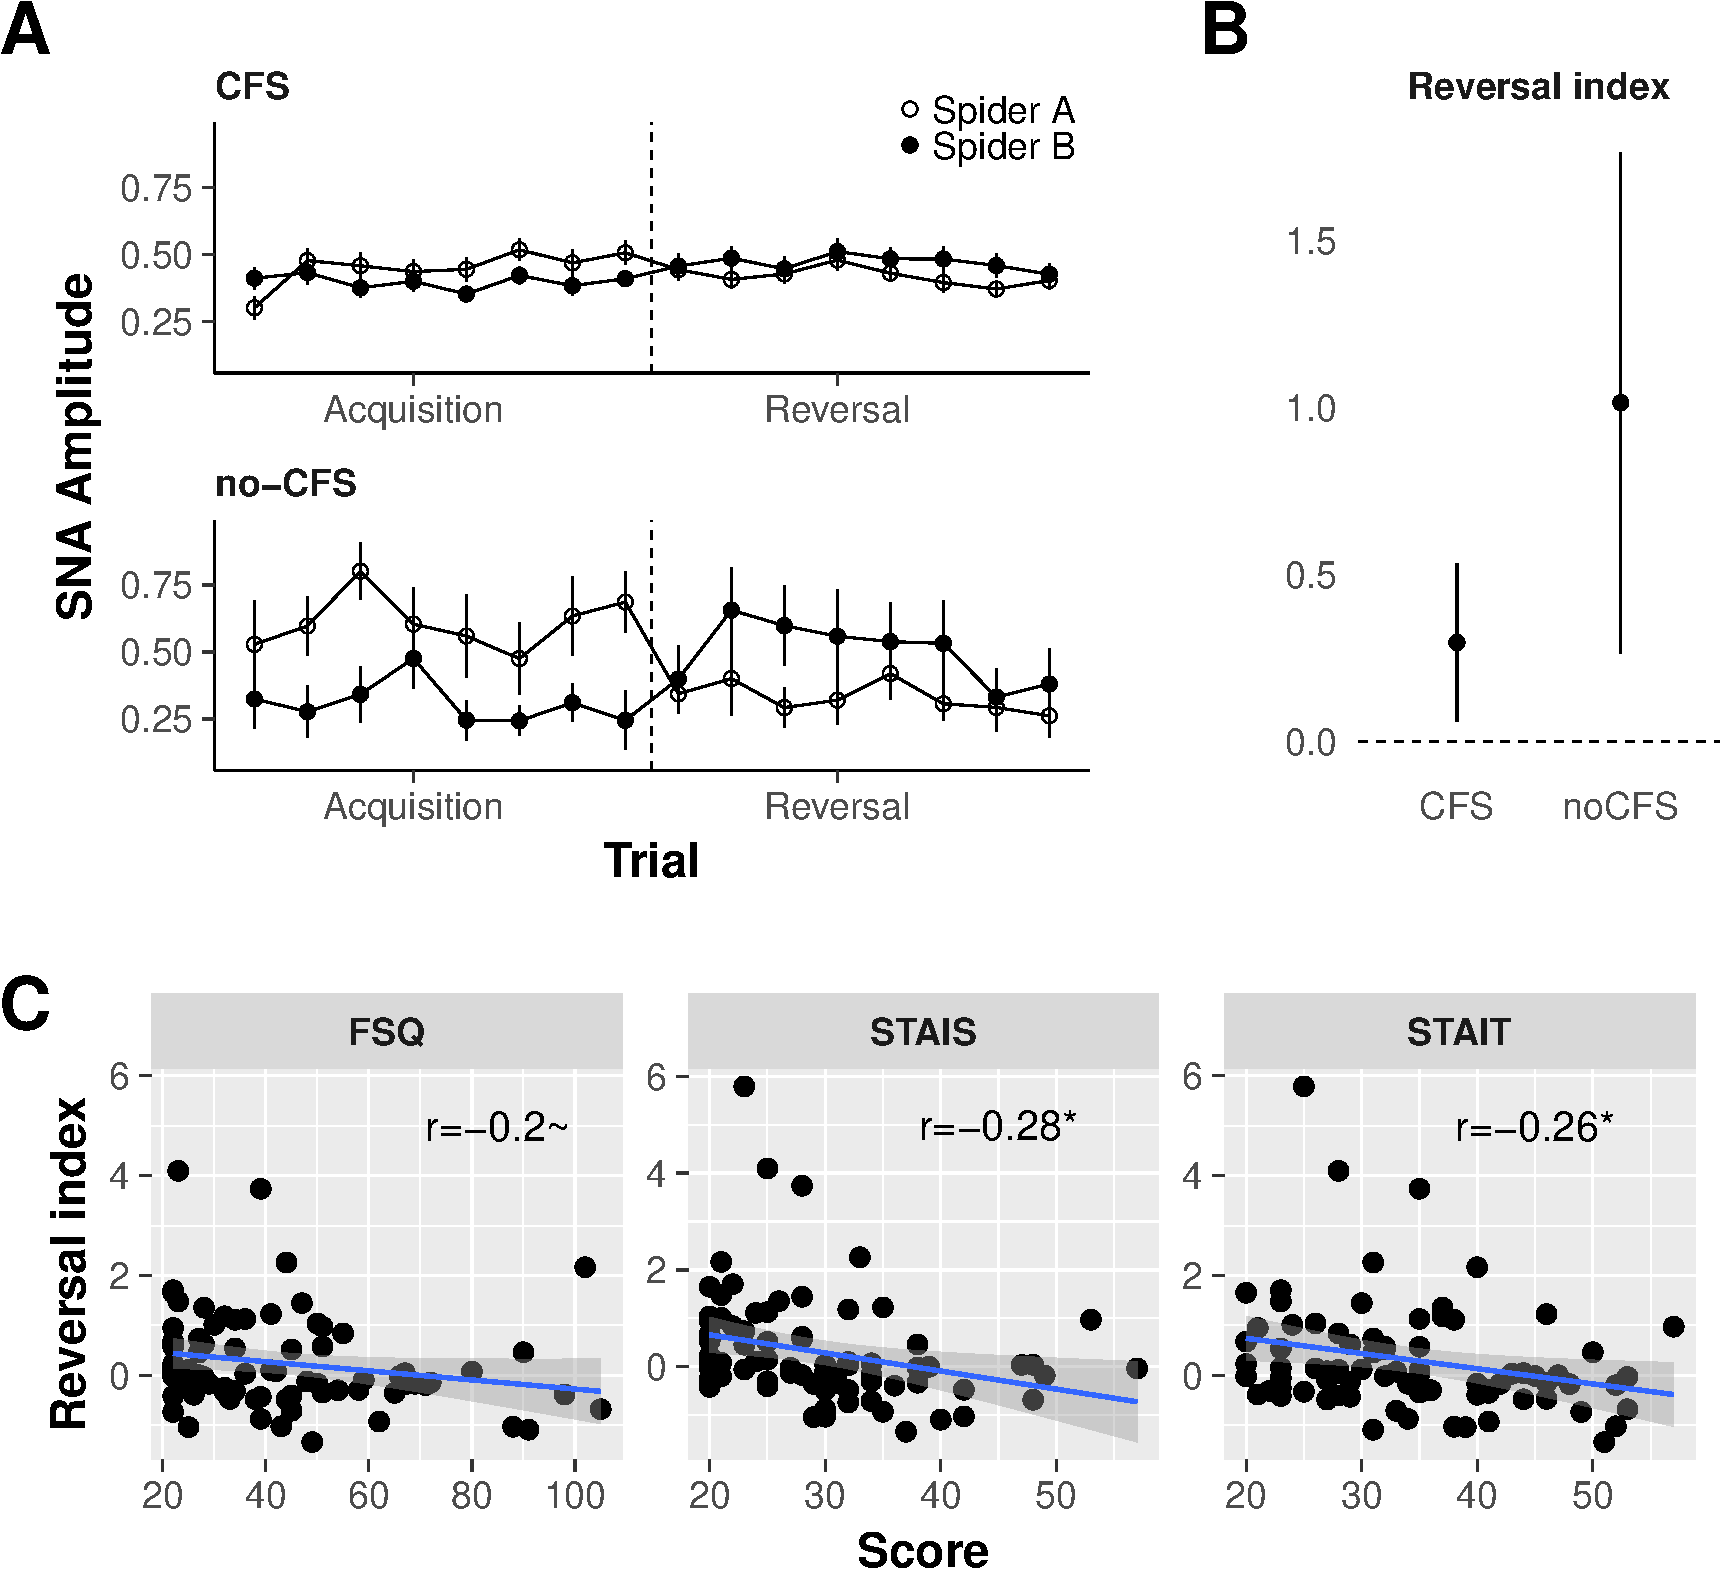
\includegraphics[width=1.0\textwidth]{cfs_timecourses-crop.pdf}
\caption{\label{fig:org8bbee4d}
\textbf{Physiological reversal} \textbf{learning.} \textbf{A. Time courses reveal reversal} \textbf{of threat responses with and without} \textbf{continuous flash suppression.} Data points represent trial-wise mean responses to spider A (the CS+ during acquisition) and spider B (the CS- during acquisition). Both groups showed evidence for reversal learning as indicated by the interaction of stage (acquisition, reversal) and stimulus (spider A, spider B) and quantified by the reversal index. Error bars represent standard errors. \textbf{B. Mean reversal learning index} \textbf{for each group.} Error bars represent 95\% confidence intervals, indicating that the interaction of stage and stimulus and thus the magnitude of reversal learning in both groups was significantly greater than zero. \textbf{C. Heightened anxiety} \textbf{is associated with impaired reversal} \textbf{learning under CFS.} A negative correlation between baseline anxiety measures and the strength of threat reversal learning is evident for state and trait anxiety. Blue lines show linear fits of each score to the reversal index, and ribbons around lines indicate bootstrapped 95\% confidence intervals around the estimate. Abbreviations: STAIS/STAIT, state/trait anxiety subscale of the Spielberger State-Trait Anxiety Inventory; FSQ, Fear of Spider Questionnaire, \textasciitilde{}, \emph{P} < .1; *, \emph{P} < .05.}
\end{figure}

\clearpage
\begin{figure}[htbp]
\centering
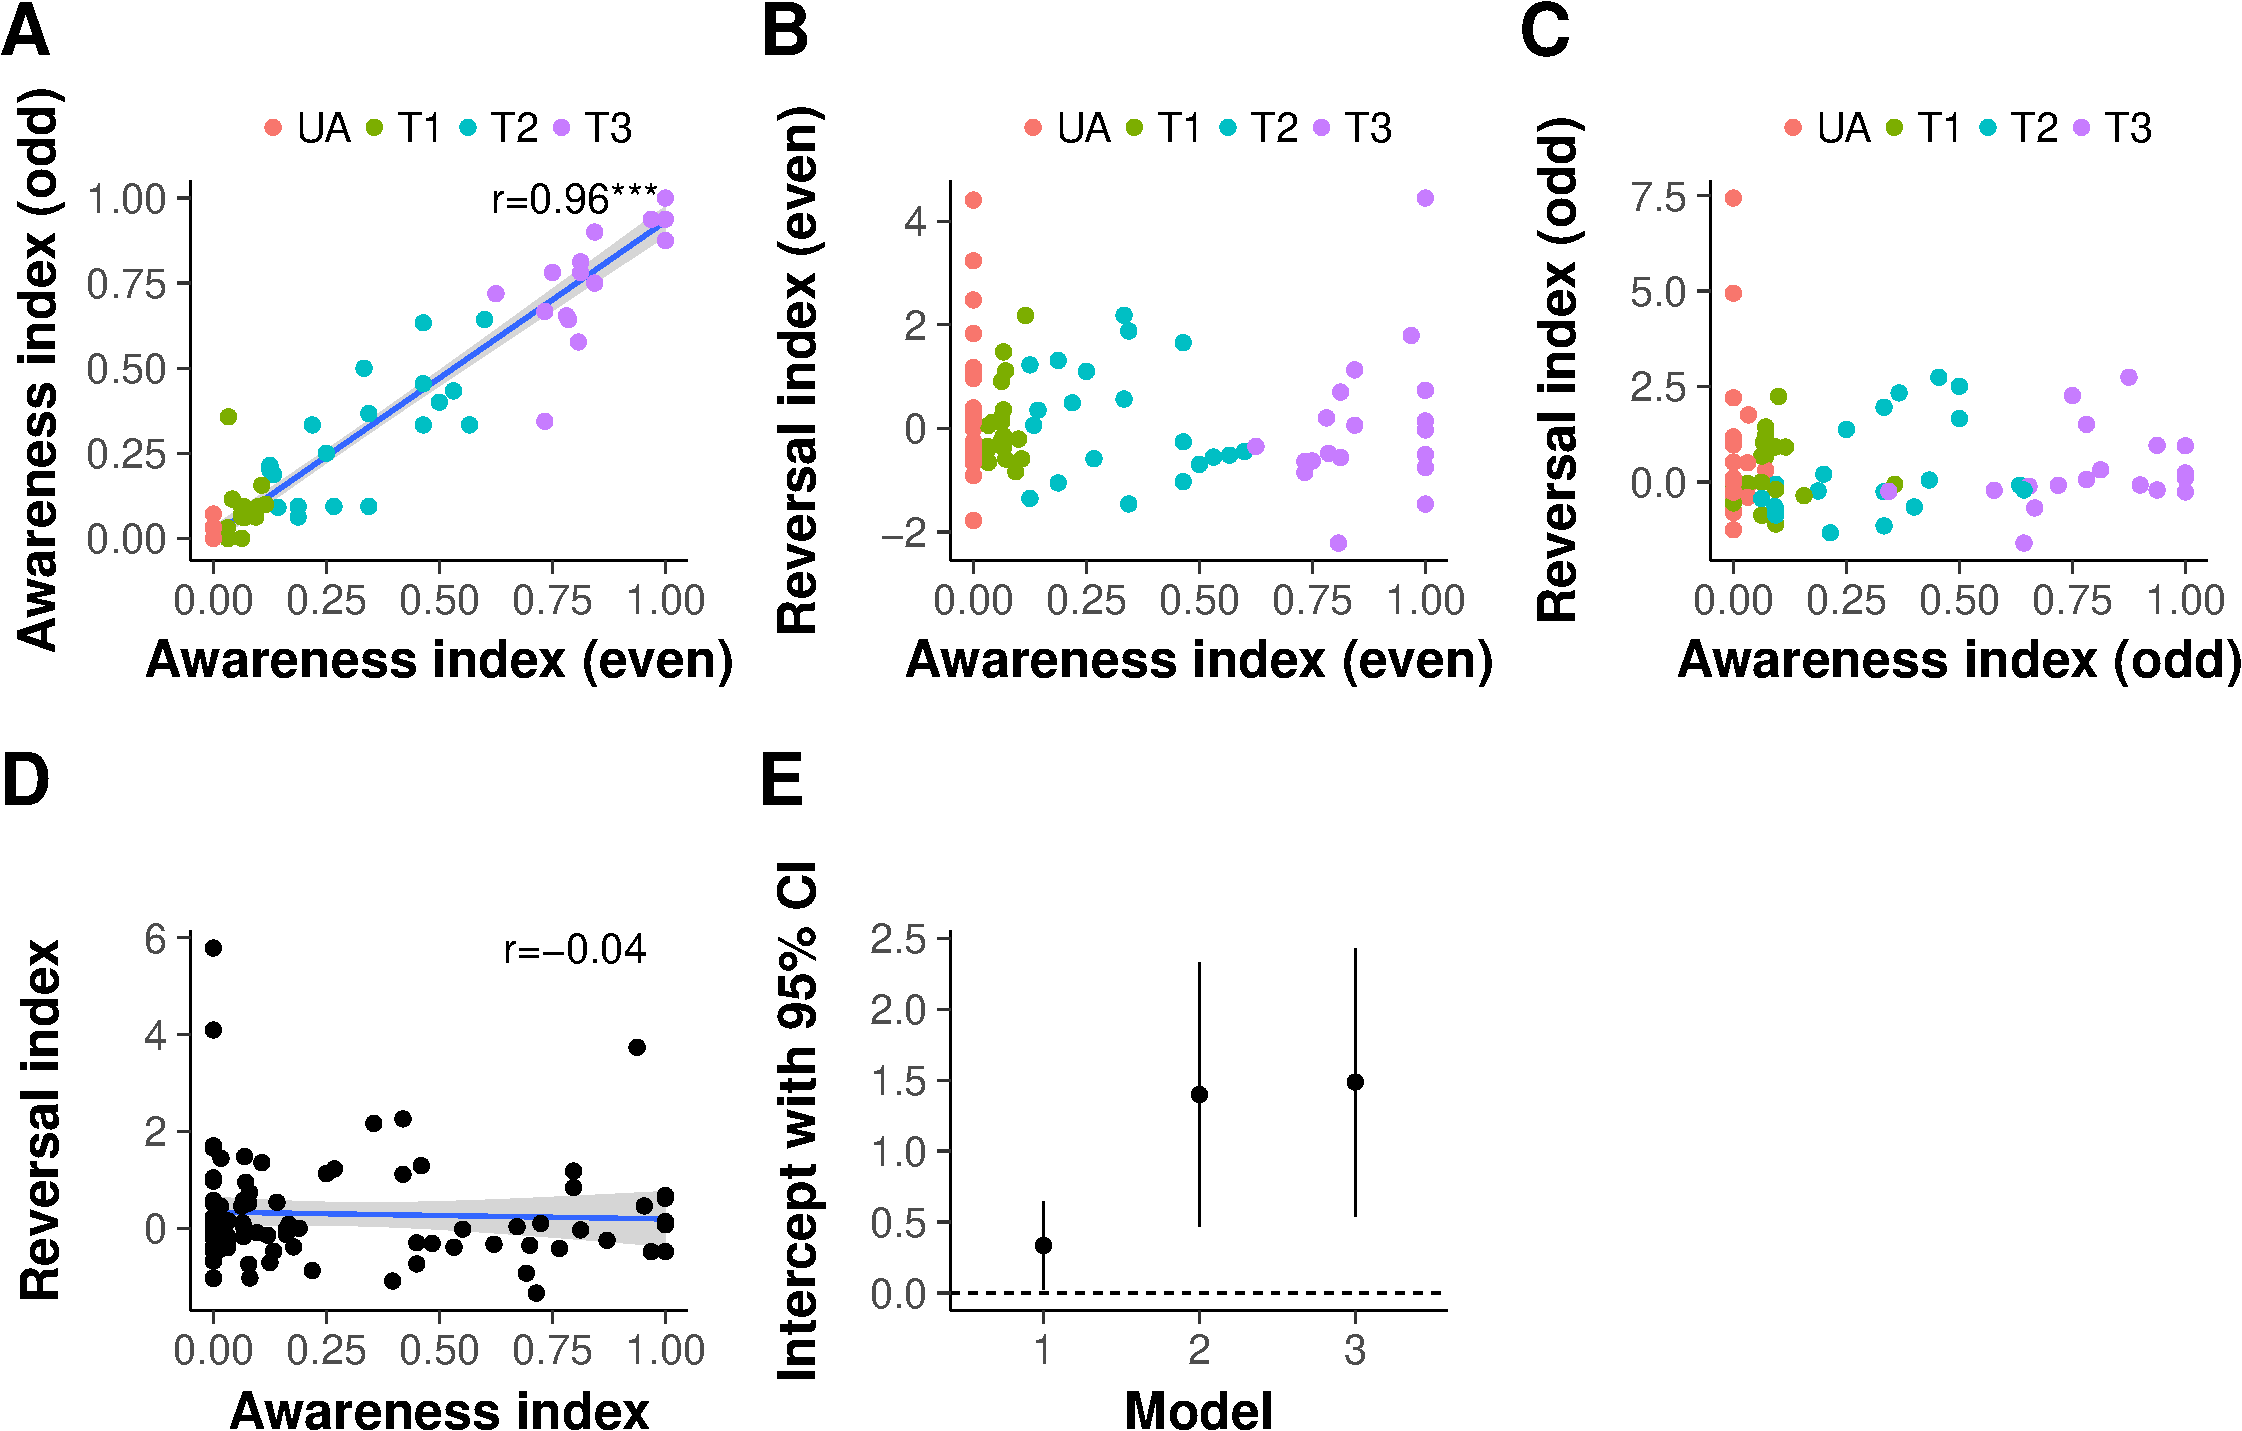
\includegraphics[width=1.0\textwidth]{cfs_regressions-crop.pdf}
\caption{\label{fig:orgd1537f6}
\textbf{Characterizing the relation between} \textbf{perceptual awareness and reversal} \textbf{learning.} \textbf{A. Correlation between the} \textbf{awareness index of even and odd-numbered} \textbf{trials.} Each data point represents an individual participant. The strong positive correlation between these independent measures of awareness demonstrates that individual participants' awareness ratings - even those with extreme values of zero or one - are unlikely to be due to measurement noise. For illustrative purposes, the color scheme marks all participants with an awareness index of 0 in even trials in red (UA, unaware, \emph{N} = 27) and classifies the rest of the sample in 3 tertiles (T1-T3). Note that some data points overlap. \textbf{B.} \textbf{Reversal learning} \textbf{plotted against perceptual awareness for} \textbf{individual participants, for data obtained} \textbf{from even-numbered trials.} The color scheme is the same as in Panel A. \textbf{C.} \textbf{Reversal learning plotted against} \textbf{perceptual awareness for individual} \textbf{participants, for data obtained from} \textbf{odd-numbered trials.} Individual participants are marked with the same color as in the previous panels; the overall distribution of participants is highly similar across panels. \textbf{D.} \textbf{Reversal} \textbf{learning as a function of perceptual} \textbf{awareness, using data pooled from all} \textbf{trials.} The intercept, indicating the magnitude of reversal learning in the absence of awareness, is positive and significantly different from zero. \textbf{E.} \textbf{Intercepts and their 95\% confidence} \textbf{intervals in a series of regression} \textbf{models.} Reversal learning is predicted by the perceptual awareness index (model 1), the perceptual awareness index and STAIT scores (model 2), and perceptual awareness, STAIT and tracking scores (model 3). (Excluding the potential outlier in the top left corner of panel D weakens significance of the intercept in model 1, \emph{P} = 0.07; the intercepts of model 2 and 3 remain significant after removal of this outlier). Blue lines show linear fits, and ribbons around lines indicate bootstrapped 95\% confidence intervals around the estimate.}
\end{figure}

\clearpage

\section*{Supplementary Information}
\label{sec:org15a3020}
\doublespacing
\setcounter{figure}{0}
\setcounter{table}{0}

\subsection*{Supplementary Methods}
\label{sec:org7456d85}
Investigating unconscious perception relies on the effectiveness of the
technique used to suppress stimuli from awareness. Although CFS is
highly effective, it is not foolproof - different observers are not
equally susceptible to it, and stimuli often break through the
suppression. The standard approach to dealing with breakthrough of the
suppressed stimulus is to remove from analysis those trials and
individuals in which it occurred. This approach is problematic, though,
as it may lead to various artifacts. Below we detail the concerns that
are addressed by the analysis approach we adopted in the present study.

\subsubsection*{Regression to the mean}
\label{sec:org072aa50}
Recent computational work suggests that findings in the trials
that remain after removing suppression failures (unless the number of
such trials is negligibly small) could be the result of regression to
the mean \cite{Shanks2016}: If two noisy measures of the same
underlying phenomenon are used (e.g., behavioral and skin conductance
responses may both measure conscious processing, each with its own,
independent measurement noise), then selecting only the extreme cases of
one measure (e.g., only those cases where behavior indicates complete
absence of awareness) is unlikely to yield similarly extreme results for
the other measure (e.g., it is unlikely that the skin conductance
responses will also be close to zero). Thus, a result that looks as if
it indicates unconscious processing would in fact be an artifact that is
entirely due to regression to the mean.

To address this issue, we refrain from removing trials or participants
with breakthrough. Instead, we include all of them in our analyses and
assess CS awareness in a continuous manner by assigning each participant
an awareness rating; we base this rating on two independent measures of
awareness (odd and even-numbered trials), as proposed by Shanks
\cite{Shanks2016} to control for regression to the mean in awareness
estimates. We then examine the association between the level of CS
awareness and the amount of reversal learning indicated by physiological
stimulus-evoked responses (Figure S\ref{fig:orge0dadc6}).

\subsubsection*{Sensitivity of awareness assessments}
\label{sec:org63c85ea}
The tasks used to assess whether participants were aware of the
suppressed stimulus (typically through examining, after each trial,
whether they can confidently and accurately report which stimulus was
presented) may not be sensitive enough to detect such awareness. This is
because breakthrough, leading to at least some awareness, may not always
reach a level that allows above-chance performance on the chosen
discrimination task (e.g., one might be able to distinguish between two
stimuli without being able to label either, a problem that falls within
the general concern of "sensitivity dissociation" between direct and
indirect measures; \cite{Stein2014a}).

To address this issue, we analyze individual participants' response
patterns across trials, searching for any link between stimuli and
behavioral responses - including consistently wrong ones - that may
indicate potential tracking of the stimuli, suggesting some perceptual
awareness (even in the absence of an explicit ability to identify the
images) and thus possibly accounting for physiological findings. We
incorporate a binary factor indicating whether or not tracking behavior
was observed in each participant into the regression model accounting
for physiological responses.

\subsubsection*{Participants expectations}
\label{sec:orgcf7b60f}
Laboratory models of conditioning require a pre-defined number of trials
for each CS category, to avoid confounding learning with exposure to
different stimulus ratios. Furthermore, the order of trials is often not
completely random but constrained to allow for roughly similar
distributions of CSs across the experiment
\cite{Schiller2008,Li2011}. This means that participants would not be
wrong to predict the probability of receiving aversive stimulation on a
given trial using a heuristic that takes into account the overall rate
of the aversive stimulus and the number of trials since its last
occurrence (this is akin to the gambler's fallacy, but in such cases has
a higher-than-chance success rate). The likelihood of participants
basing their anticipation of a shock - and of the physiological arousal
that comes with such anticipation - on such probabilistic estimates may
be even higher when CSs are suppressed from awareness, leaving the
overall rate and distribution of shocks as the only bases for such
predictions. We address this issue by we using Bayesian model
comparison, demonstrating that a model featuring updating of learning
account for the findings better than a shock-expectation model based on
the distribution of shocks across the experiment.

\clearpage
\singlespacing

\singlespacing
\begin{table}[htbp]
\centering
\begin{tabular}{lrrrrrr}
\textbf{Characteristic} & \textbf{N (CFS)} & \textbf{Mean} & \textbf{SD} & \textbf{N (no-CFS)} & \textbf{Mean} & \textbf{SD}\\
\hline
Male & 38 & nil & nil & 7 & nil & nil\\
Female & 48 & nil & nil & 5 & nil & nil\\
Age, y & 86 & 29.7 & 8.3 & 12 & 31.7 & 10.6\\
STAIT & 80 & 34.2 & 9.6 & 11 & 33.5 & 12.3\\
STAIS & 80 & 29.4 & 8.6 & 11 & 28.4 & 9.2\\
FSQ & 79 & 43.5 & 21.5 & 12 & 36.8 & 12.1\\
UR, SNA units & 86 & 1.8 & 0.5 & 12 & 1.8 & 0.7\\
\end{tabular}
\caption{\label{tab:org270f0e5}
\textbf{Sample characteristics.} Note: STAI data for 7 participants (6 in the CFS condition) and FSQ data for 7 participants (all in the CFS condition) were lost due to an archiving error. Exclusion of these participants from subsequent analyses does not alter the overall pattern of results. \emph{Abbreviations}: CFS, Continuous Flash Suppression; SD, Standard deviation; STAIS/STAIT, state/trait anxiety subscale of the Spielberger State-Trait Anxiety Inventory; FSQ, Fear of Spider Questionnaire; UR, unconditioned response (shock response); SNA, sudomotor nerve activity.}

\end{table}

\clearpage

\begin{figure}[htbp]
\centering
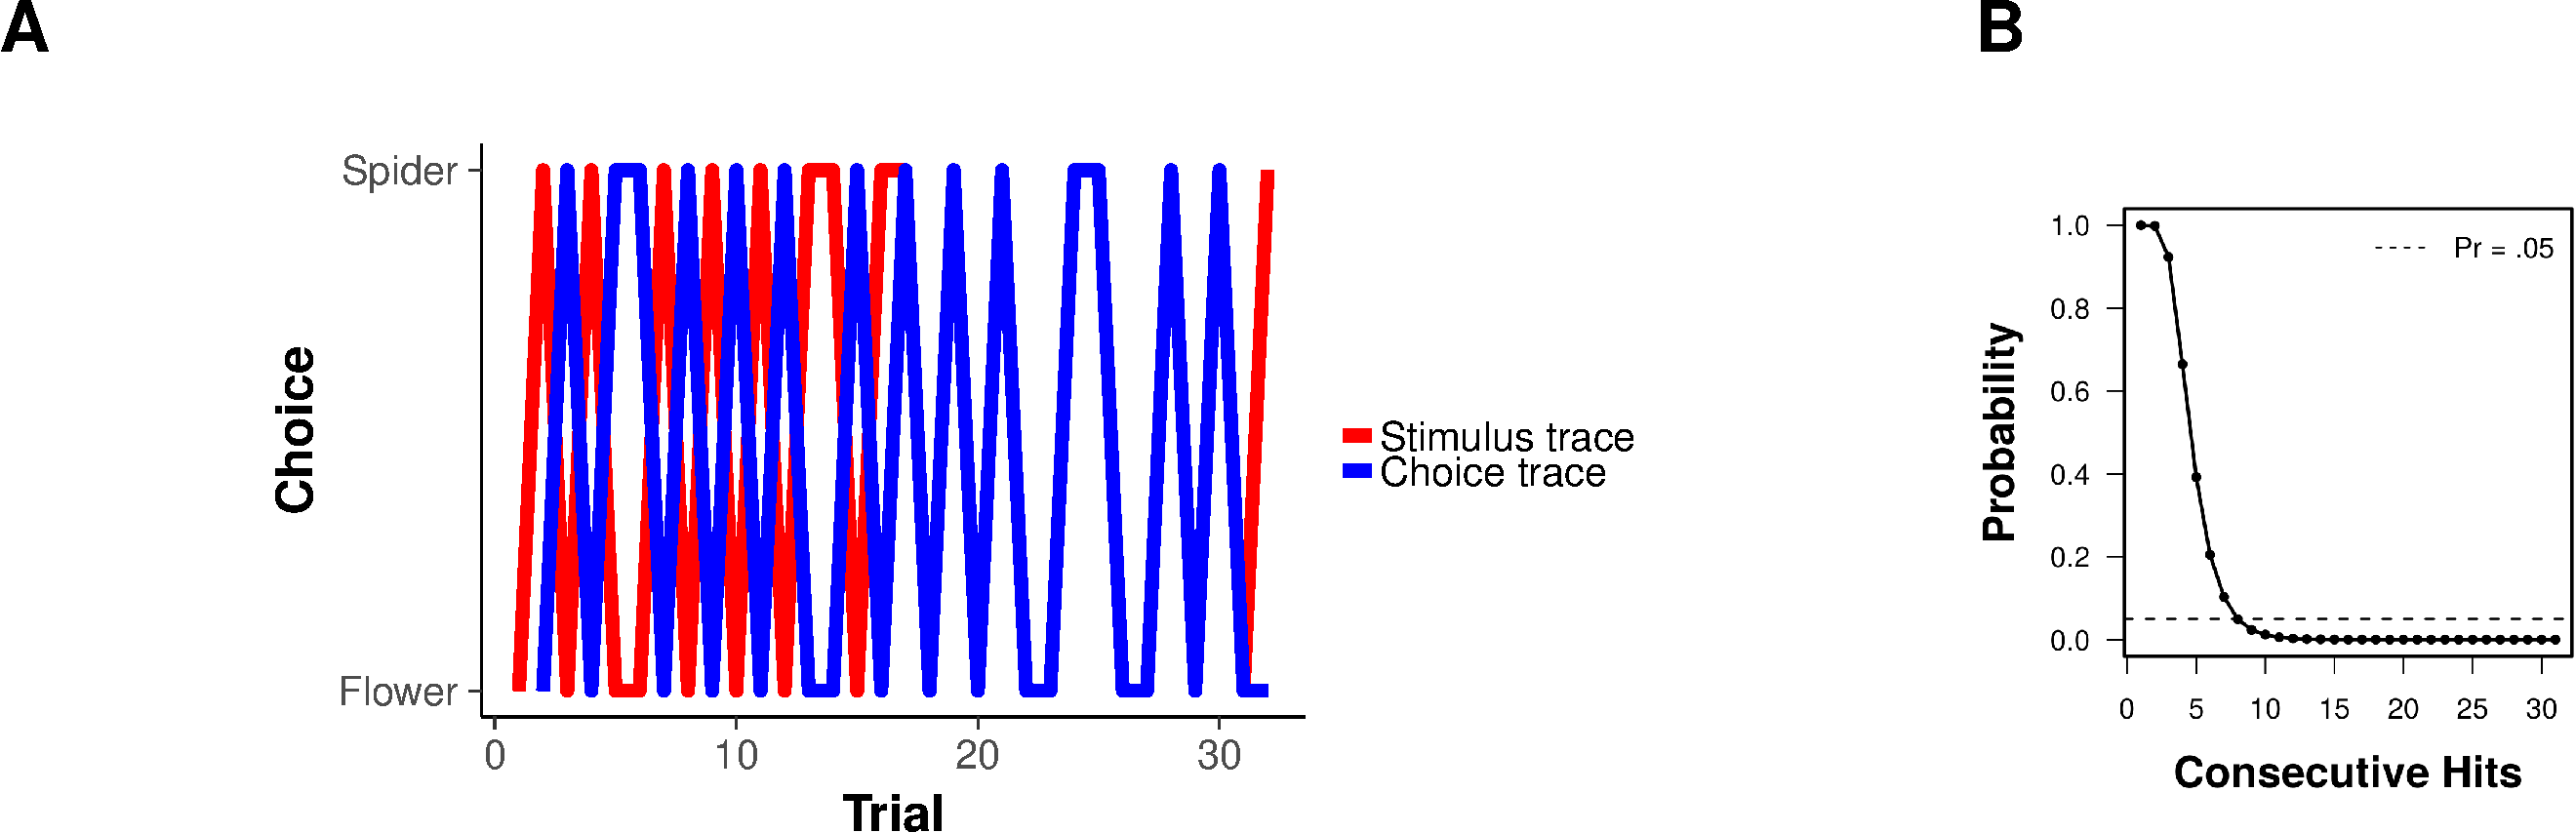
\includegraphics[width=1.0\textwidth]{cfs_sub_binomsim-crop.pdf}
\caption{\label{fig:orge0dadc6}
\textbf{Examination of tracking behavior in the} \textbf{correspondence between time courses of} \textbf{forced-choice responses and stimulus} \textbf{presentation in} \textbf{the CFS group.} \textbf{A.} \textbf{Forced choice responses} \textbf{(blue) versus stimulus presentation (red)} \textbf{in an illustrative participant.} This participant shows periods in which forced-choice responses track or are in direct opposition to both the presented stimuli and shock application, suggesting that this participant tracked the spider and/or the shock with his responses. \textbf{B.} \textbf{Probability} \textbf{of consecutive hits (10\(^{\text{5}}\) simulations).} Hits were defined as the number of consecutive trials where the time courses of forced-choice responses and stimulus presentation were either identical or directly opposed to each other. To quantify the probability of consecutive hits, we simulated the probabilities for all possible levels of consecutive hits (e.g., from 1 to 31 for 32 trials). We simulated 10\(^{\text{5}}\) draws of a binomial distribution, and calculated the average probability to see (at least) each possible number of consecutive hits. The probability exponentially declines as the number of consecutive hits increases, reaching a probability of about 5\% at 8 consecutive hits. Thus, observing 8 or more consecutive hits in 32 trials in a perceptually unaware participant who is truly guessing is unlikely, which is why we considered this an indication for stimulus tracking behavior.}
\end{figure}

\clearpage

\begin{figure}[htbp]
\centering
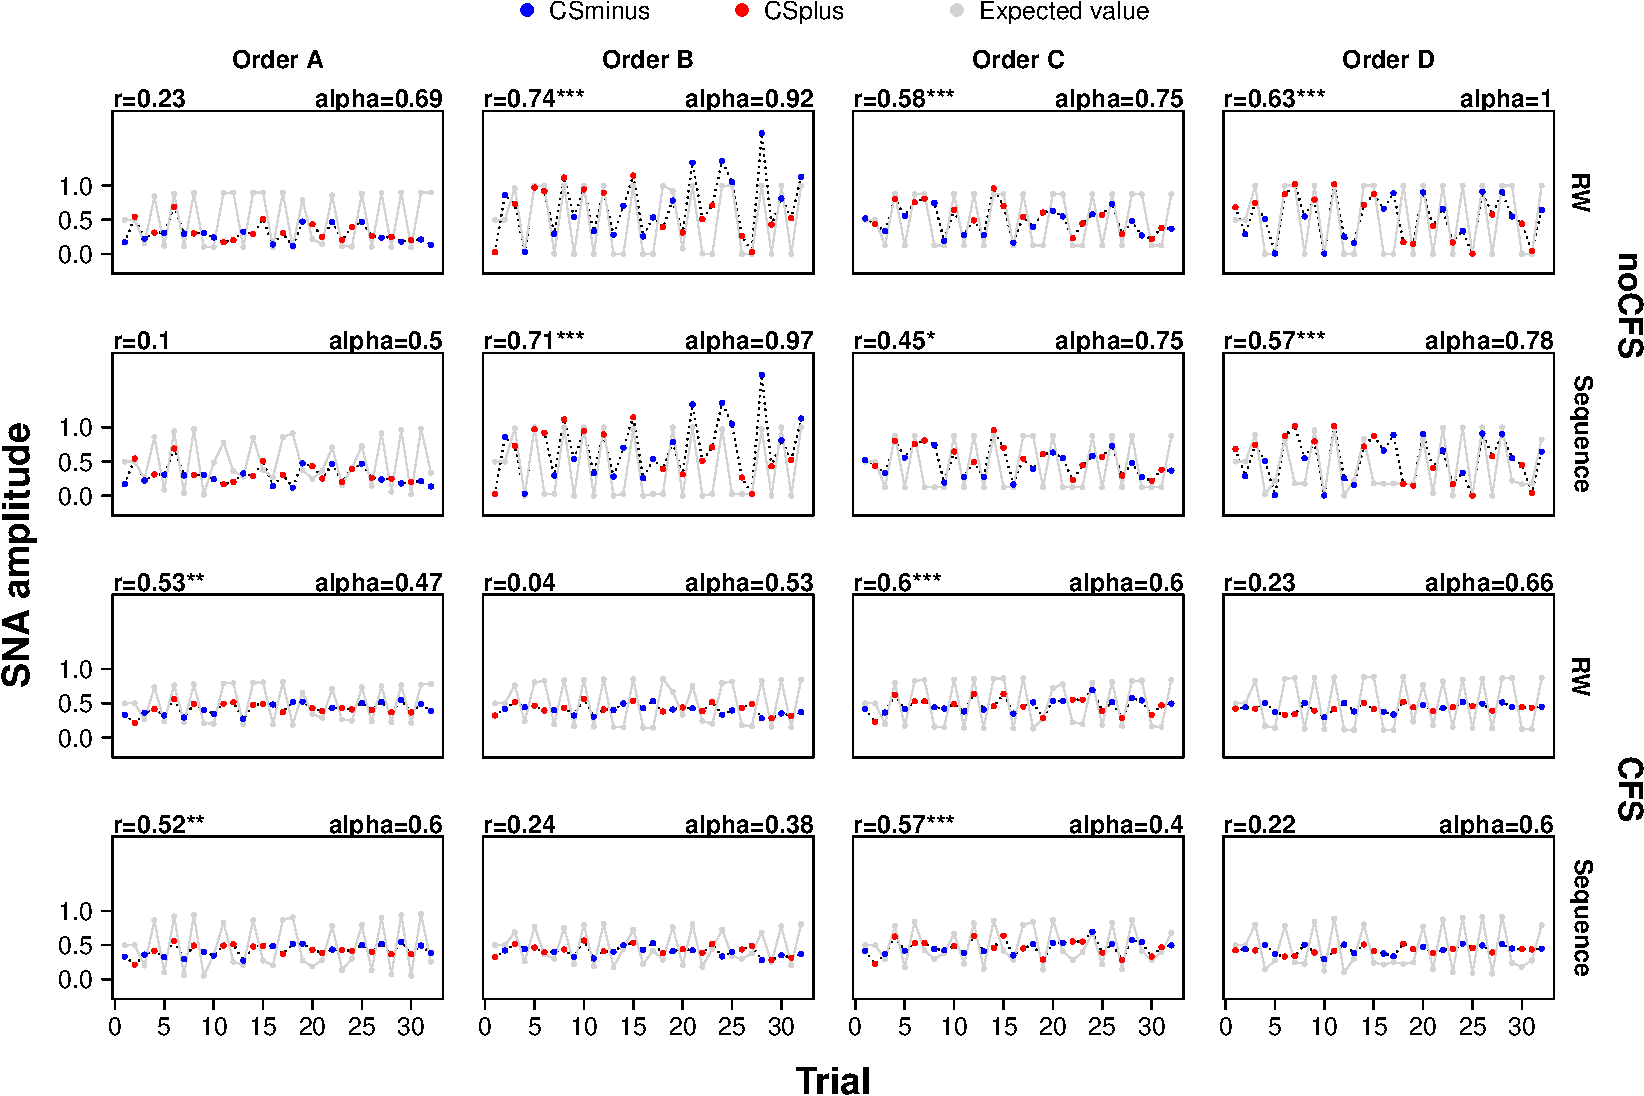
\includegraphics[width=1.0\textwidth]{cfs_modelfits-crop.pdf}
\caption{\label{fig:org918e8f8}
\textbf{Time series of measured and predicted} \textbf{threat response indicate that the} \textbf{Rescorla-Wagner learning model explains} \textbf{the data better than an alternative} \textbf{trial-sequence learning model that simply} \textbf{assumed a sequence of alternating trial} \textbf{types (no-shock/shock or vice} \textbf{versa).} Trial-wise mean responses to CS+ and CS- are shown by group, learning model and experimental order. Each panel also shows the Pearson correlation between predicted and measured time series and the learning rate (parameter alpha in each of the learning models). The generally higher Pearson correlation coefficients are consistent with the formal model comparison between the Rescorla-Wagner model and the trial-sequence model, which confirmed that the Rescorla-Wagner model provided stronger evidence than the alternative learning model. r, Pearson correlation coefficient; alpha, learning rate; RW, Rescorla-Wagner learning model; Sequence, trial-sequence learning model; SNA, sudomotor nerve activity; \textbf{*}, \emph{P} < 0.001; **, \emph{P} < 0.01; *, \emph{P} < 0.05.}
\end{figure}
\end{document}
